% vim:spell:spelllang=en_us
\documentclass[a4paper]{IEEEconf}

\usepackage{tikz}
\usepackage[utf8]{inputenc}
\usepackage[T1]{fontenc}
\usepackage{listings}
\usepackage{graphicx}
\usepackage[caption=false]{subfig}


\lstset{language=C} 
\lstset{basicstyle=\footnotesize} 
\lstset{tabsize=2} 

\makeatletter
\newbox\sf@box
\newenvironment{SubFloat}[2][]%
  {\def\sf@one{#1}%
   \def\sf@two{#2}%
   \setbox\sf@box\hbox
     \bgroup}%
  { \egroup
   \ifx\@empty\sf@two\@empty\relax
     \def\sf@two{\@empty}
   \fi
   \ifx\@empty\sf@one\@empty\relax
     \subfloat[\sf@two]{\box\sf@box}%
   \else
     \subfloat[\sf@one][\sf@two]{\box\sf@box}%
   \fi}
\makeatother


\title{Heißes Eisen: Discovering the Properties of a Soldering-Iron Tip
and Building a Matching Soldering Station}
%Heisses Eisen: Building an Open Source Soldering Station for COTS Tips
\author{%
	Philip Feuerschütz\\
	Arne Jünemann\\
	Sven Mattsen\\
	Arne Wichmann\\
}

\begin{document} 
\maketitle{}
\begin{abstract}
Professional Soldering Stations impose a high financial burden for
electronics hobbyists. Some Commercial Tips with integrated
heating- and thermal-elements use connectors that can be used with
standard sockets. Heißes Eisen describes the process of discovering the
thermal-element parameters and the build process of a
temperature-controlled soldering station.
\end{abstract}

\part{Soldering-Iron Tip}
% vim:spell:spelllang=en_us
\section{mechanical tip properties}
Weller WMRP tip "RT 3" 1,3x0,4mm
approx 10cm
tip, heater, sensor, grip, 3,5mm jack
nominal 


\section{thermal element}


\subsection{common element types}
type K -> tried AD8495 AR: $5mV/\deg C$ output
other types: very unlikely


\subsection{custom measurement amplifier}
to accurately measure the thermocouple voltage and to record the tips characteristics, an amplifier has to satisfy the following conditions:
- Very high input resistance (thus very low input current) because of the t/cs low impedance
- very low offset to be able to amplify signals in the microvolt-range
- rail-to-rail input and output, because of low input voltage and 5V supply
- high linearity (low gain error)

AD 8552 AR
provides:
 - $1\,\mu V$ offset
 - $0,005\,\mu V/\deg C$ drift


With the AD 8552 a simple non-inverting amp was constructed. Gain was trimmed to $g=400$.

Previously constructed AD8495 circuit was used to provide reference temperature information.

WMRP Tip, reference type K thermocouple were closely thermally coupled to another soldering iron. An Atmel Atmega8 MCU with an 10bit ADC was used to record data.

First results showed a linear dependence of thermocouple voltage and temperature in a range of 150-250 $\deg C$ with a coefficient of about $16\,\mu V/K$.


\section{heating element}

\part{Soldering Station}
% vim:spell:spelllang=en_us

\section{system overview}



\subsection{UI}
\paragraph{Functional Requirements}

\begin{itemize}
	\item Show the real and control temperature of the tip.
	\item Allow an arbitrary change of temperature by interaction
		with a single UI element.
	\item Provide (with additional systems) the ability to monitor
		the system and set control parameters.
\end{itemize}
\paragraph{Interface Components}
\begin{itemize}
	\item Rotary encoder.
	\item 7-Segment display.
	\item Serial (USB) debug line.
\end{itemize}

\section{temperature control}

\section{performance evaluation}





\end{document}


\section{Executables}
\subsection*{Why analyze Executables?}

This work presents the methods used in the \mbox{DIVINE} (DIscovering Variables IN
Executables) analysis to give precise information about the variable-like entities that
can be found in executables.


There are several possible users of such an analysis, including the
intelligence community, anti-virus companies, hackers of all shades, computer
emergency/incident response teams (CERTs) and common reverse engineers. All of
them want to analyze executables directly but have very different reasons to do
so. 

The simplest case is the unavailability of the source code of a particular
executable. This might simply be lost code, which the reverse engineer
has to recover,
or the analysis of malware, when analyzing the workings of an exploit or the
intentions of the author, or the components of an operating system when looking
for possible bugs and exploits, just to name some possibilities.
%
Another motivation to analyze executables is the mistrust in the tools used in
the development process of an application. This might be the introduction of
new and hidden functionality by some component used in the construction process
or the analysis whether there is any unintended functionality.

The analysis of executables is also interesting because in the final
executable, there usually is a significantly reduced number of paths in the
control-flow graph compared with the original source code.

The given intentions for the analysis imply that all kinds of software is
analyzed on executable level. Obviously, this is malware, as well as Commercial Of
The Shelf (COTS) software, but also in-house software in case of mistrust in
the tools used.


To describe the functionality of an executable, information about the
control-flow and variable access is needed.
When analyzing executables it is relatively easy to give information about
directly addressed variable access or program jumps. The frame-relative
addressing on the stack is also fairly easy to handle.
Indirect addressing of memory is a problem, because it is not trivial to know
what the contents of a register or of a memory location may be that is
used for addressing.

\mbox{DIVINE} discovers variable-like entities in executables.  It does not give
information about the program's control flow. It can provide information about
indirect jumps and indirect function calls.


Nearly all of this information could be extracted from the executable
debug information, but the executable may be stripped of this information or
the debug information might be untrusted, as it might be intentionally
describing another behavior as the actual code is implementing.

%\enlargethispage{5\baselineskip}
\subsection{x86 Assembler}
\enlargethispage{2\baselineskip}

To understand the \mbox{DIVINE} analysis it is necessary to understand
the basic concepts of an assembly language. This work uses the x86
assembly language because it is widely deployed and the current
\mbox{DIVINE} implementation (Codesurfer/x86) can only analyze x86
executables at the moment. The concepts, however, are of general nature
and can be applied to other assembly languages as well. 

First, it is described what kind of addressing is possible. Second, the
typical locations of variables in the memory are discussed.


\subsubsection{x86 Addressing Modes}

X86 provides a versatile set of addressing modes used to access variables.
The discussion focuses on the possible addressing modes of the \verb+mov+ instruction,
because it simply copies data from one location to another and no further
consideration except the memory/data access is necessary.

\begin{table}[!h]
	\begin{tabular}[h]{l l l}
		\lstset{language=[x86masm]Assembler,xleftmargin=0pt}
		\lstinline+mov  %edx, %ecx+&$\iff$& 
		\lstset{language=C,xleftmargin=0pt}
		\lstinline+ecx=edx;+\\& & register to register\\
	\lstset{language=[x86masm]Assembler,xleftmargin=0pt}
		\lstinline+mov  (%edx), %edx+&$\iff$& 
		\lstset{language=C,xleftmargin=0pt}
		\lstinline+ecx=*edx;+\\& & indirect to register\\
	\lstset{language=[x86masm]Assembler,xleftmargin=0pt}
		\lstinline+mov  %edx, (%ecx)+&$\iff$& 
		\lstset{language=C,xleftmargin=0pt}
		\lstinline+*ecx=edx;+\\& & register to indirect\\
	\lstset{language=[x86masm]Assembler,xleftmargin=0pt}
		\lstinline.mov  (%edx+8), %ecx.&$\iff$& 
		\lstset{language=C,xleftmargin=0pt}
		\lstinline+ecx=&a[2];+\\& & ind.\ with computation\\
	\lstset{language=[x86masm]Assembler,xleftmargin=0pt}
		\lstinline+mov  $0x123, %ecx+&$\iff$& 
		\lstset{language=C,xleftmargin=0pt}
		\lstinline+ecx=*(0x123);+\\& & absolute to register\\
	\end{tabular}
	\caption{x86 Addressing for the \texttt{mov} Instruction}
	\label{tab:mov-addressing}
\end{table}

Table \ref{tab:mov-addressing} shows the different addressing possibilities of
the \verb+mov+ instruction. (GNU-assembler semantics is used: Source first,
then destination.)

The simplest addressing mode possible is the movement of data from one register to
another. No memory access out of the CPU is necessary. It is easy to track.
More complex addressing is possible, when the \verb+mov+ instruction is used
with one indirect operand. (The use of two indirect operands is prohibited.)
This allows to read from memory into a register or write the contents of a
register into memory.  It is possible to use indirect addressing in a very
complex manner: \verb+offset(%base, %index, scale)+ (\verb+%base+ and
\verb+%index+ are registers. \verb+scale+ and \verb+offset+ are constants.)
This allows addressing of structures like arrays and structs with one
instruction.
The last addressing mode is absolute addressing, where an address is given
during the assembly phase and fixed during all executions. It can only address
global and static variables and its analysis is simple.


% 1. adressing modes

\subsection{Home of Variables} 
\enlargethispage{2\baselineskip}

It is important to know the common locations of variables in the machines
memory.  Variables can exist in the activation record, as global or static
variables, or on the heap.  Details about the types of variables and their
corresponding implementation in the assembler code follow.

The compiler assigns fixed addresses to global and static variables during the
compilation.  Global and static variables are very simple to locate in the
assembler code.  They are addressed with an absolute address by the compiler
and have a fixed position in the program memory.

Heap variables are created during the runtime of the program, inside a memory
region called the heap.  Tracking the heap is difficult. It is not
possible to see from a simple analysis where the memory will be located and how
much memory is actually allocated. Looking at the assembler code one will only
notice some memory location that is used to store the address of some other memory location.
To give any useful information it is necessary to know what possible values are
contained in the first location and what can be used as an address.

%\subsubsection<article>{Global and Static Variables}
%\begin{figure}[!h]
%\centering
%\begin{minipage}{0.45\textwidth}
%\centering
%\begin{lstlisting}
%int a;
%
%void bar(void) {
%	static int b;
%	b=a;
%}
%\end{lstlisting}
%\end{minipage}
%\begin{minipage}{0.45\textwidth}
%\centering
%\begin{lstlisting}[numbers=left,language={[x86masm]Assembler}]
%bar:
%	pushl   %ebp
%	movl    %esp, %ebp
%	movl    a, %eax
%	movl    %eax, b
%	popl    %ebp
%	ret
%\end{lstlisting}
%\end{minipage}
%\end{figure}


%\subsubsection<article>{Heap-Variables}
%\begin{figure}[!h]
%\centering
%\begin{minipage}{0.29\textwidth}
%\centering
%\begin{lstlisting}
%int *p;
%
%void foo(void) { 
%	p=malloc(123);
%}
%
%void bar(void) { 
%	free(p); 
%}
%\end{lstlisting}
%\end{minipage}
%\begin{minipage}{0.39\textwidth}
%\centering
%\begin{lstlisting}[numbers=left,language={[x86masm]Assembler}]
%foo:
%	pushl   %ebp
%	movl    %esp, %ebp
%	subl    $24, %esp
%	movl    $123, (%esp)
%	call    malloc
%	movl    %eax, p
%	leave
%	ret
%\end{lstlisting}
%\end{minipage}
%\begin{minipage}{0.3\textwidth}
%\centering
%\begin{lstlisting}[numbers=left,language={[x86masm]Assembler}]
%bar:
%	pushl   %ebp
%	movl    %esp, %ebp
%	subl    $24, %esp
%	movl    p, %eax
%	movl    %eax, (%esp)
%	call    free
%	leave
%	ret
%\end{lstlisting}
%\end{minipage}
%\end{figure}


\subsubsection{Activation Record}

\enlargethispage{1.5\baselineskip}
The local variables, allocated during runtime on the call stack are relatively
easy to track.  
When a function is called, its activation record is put on the
stack. The layout of the activation record is determined during the compilation
phase of the program.  The x86 architecture provides a simple method to build a
call stack with a stack- and a basepointer. The stackpointer keeps track of
activation records, pointing to the end of the activation record. The
basepointer points to the beginning of the activation record, and allows
relative addressing of local variables.

\begin{figure}[!h]
	\centering
	\subfloat[C Code]{
	\begin{minipage}{0.5\columnwidth}
	\lstinputlisting[language=C]{ex1/ex.c}
	\end{minipage}
	}
	\subfloat[Assembly Code]{
	\begin{minipage}{0.5\columnwidth}
	\lstset{language=[x86masm]Assembler}
	\lstinputlisting[name=ex1s,linerange={5-16}, numbers=left]{ex1/ex.s}
	\end{minipage}
	}
	\\
	\subfloat[Layout of Activation Record]{
	\begin{minipage}{\columnwidth}
	\centering
		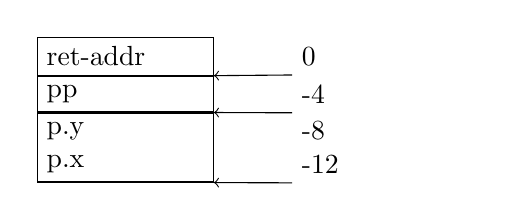
\begin{tikzpicture}
			\matrix (ar_main) [nodes={text width=2cm}, column sep=1cm] {
			\node (ret) [draw] {ret-addr}; \pgfmatrixnextcell
			\node (a0) {0}; \\
			\node (pp) [draw] {pp}; \pgfmatrixnextcell
			\node (a4) {-4}; \\
			\node (p) [draw] {p.y\\p.x}; \pgfmatrixnextcell
			\node (a12) {-8\\-12}; \\
			};
			\draw [->] (a0.south west) -- (ret.south east);
			\draw [->] (a4.south west) -- (pp.south east);
			\draw [->] (a12.south west) -- (p.south east);
		\end{tikzpicture}
	\end{minipage}
		}
	\caption{Simple Example of Stack-Relative Addressing}
	\label{fig:stack-relative}
\end{figure}

\callout{Figure \ref{fig:stack-relative}} shows a simple function written in C, the
layout of the corresponding activation record and the assembler code of the
function. Assembler lines 2-4 form the function preamble. It saves the old
basepointer on the stack, updates the basepointer using the stackpointer and
``allocates'' new memory on the stack by decrementing the stackpointer.
%
In lines 5 and 6 the location -4 relative to the basepointer is initialized
with the address -12 relative to the basepointer. This represents the
initialization of the \texttt{pp} pointer.
%
In lines 7,8,9 the address saved in \texttt{pp} is read and the memory it set
to 1 without an offset and to 2 with the offset of 4, representing the
initialization of the point \texttt{p}.
%
Lines 10,11,12 move the value of \texttt{pp->y} into the register
\texttt{\%eax} and leave the function.

% 2. c fkt in asm
%stack-pointer, activation record

\section{Basic Concepts}

This section introduces the basic executable analysis called semi-naïve
approach and asks the question what level of detail is necessary in the
analysis output.

\begin{figure}[!h]
	\centering
	\subfloat[C Code]{
	\begin{minipage}{0.5\columnwidth}
\lstinputlisting[xleftmargin=-6pt,language=C]{ex2/ex.c}
\end{minipage}
}\subfloat[Assembly Code]{
	\begin{minipage}{0.4\columnwidth}
\lstset{language=[x86masm]Assembler} \lstinputlisting[xleftmargin=0pt,linerange={5-19}, numbers=left]{ex2/ex.s}
\end{minipage}
}
\caption{Advanced Example with Loop}
\label{fig:ex-loop}
\end{figure}

\subsection{The Semi-Naïve Approach}

\lstset{language=[x86masm]Assembler}

The semi-naïve approach addresses the basic types of variables. It is able to
locate the global and static variables that are addressed with an absolute
address (%
\lstinline|movl    $0x1234, %eax|  
). It is also able to cope with stack-pointer \lstinline+%esp+ or base-pointer
\lstinline+%ebp+ relative addressing.
It is not able to recover the variables that are addressed using general
relative addressing.

Looking at the example in \callout{Figure \ref{fig:stack-relative}} the semi-naïve
algorithm is able to locate two variables. From instruction 5, it knows that one variable starts at \lstinline+-12(%ebp)+. Instruction 7 gives the
information that one variable exists at \lstinline+-4(%ebp)+.
The algorithm is not able to give the subdivision of the variable starting at -12 on the
stackframe.



\subsection{Arrays and Structs or Granularity and Expressiveness}

\enlargethispage{2\baselineskip}
The semi-naïve algorithm is not able to give subdivisions of structure entities.
This leads to the question, what level of subdivision is necessary for an
analysis to be useful.

% unions?


\callout{Figure \ref{fig:ex-loop}} is an extended example, which initializes an array of
5 points with the values 1 and 2 as x and y members.

\lstset{language=C}
The semi-naïve approach will be able to locate the variables var\_36, var\_40.
This is not a helpful subdivision, as the variable \lstinline|p[0].y| is
split off the rest of the array, which is not subdivided any more than this.
%
A better subdivision would be the set of all the members of the structure for
each entry of the array: \lstinline|p[0].x, p[0].y, p[1].x, ..., p[3].y, p[4].x, p[4].y|.
%
The best subdivision would recognize that the executable analyzed uses an
array of a certain length and has two members for each array entry: \lstinline|p[?].x, p[?].y|


\section{Building the Analysis}
This section describes the algorithms needed to build the \mbox{DIVINE} analysis.
The first part describes the concept of abstract locations, followed by rough
descriptions of the value-set analysis (VSA) and aggregate structure
identification (ASI).
The section ends describing how the \mbox{DIVINE} algorithm is built using VSA
and ASI.

\subsection{Regions and A-locs}
%one slide

It is not possible to consider the address space of an executable as a single
linear address space. This problem is given by two simple observations:

First, an address may be used by more than one variable. For example on the stack it
is possible that the creation of a new activation record used the same
addresses for its variables that were uses by another activation on the stack
that is no longer active.

Second, a variable may occur at more than one address. Local variables of a function
recursively calling itself can occur on more than one position on the stack at
the same point of time with possibly different contents. 

Memory regions represent the places in memory where variables, stripped
off their offset in memory, occur. Typical memory regions are the global
address scope, the activation record address space of a particular
function, and the heap allocation address space.

Abstract locations (\mbox{a-loc}s) divide a memory region into variable-like
entities. \mbox{A-loc}s may also represent the content of a register. They are the
abstract concept used to represent the memory and registers of the machine that
the executable is running on.


\subsection{Value-Set Analysis (VSA)}
\enlargethispage{2\baselineskip}

VSA is a flow-sensitive algorithm that keeps track of all possible
values of all \mbox{a-loc}s of a program.
It extracts information about updates to \mbox{a-loc}s. This is needed to be
able to track indirect operations, as \mbox{a-loc}s may be used to store
locations of other \mbox{a-loc}s.
Knowing what possible values an \mbox{a-loc} can contain, it gives information about
indirect memory operands, functions calls and jumps that use the \mbox{a-loc}'s
value as their operand.

VSA also generates data-access constraints to be used with ASI (Aggregate
Structure Identification). Data-access constraints describe the movement of
data from one \mbox{a-loc} to another, specially considering the width of the
movement (byte, word, etc.\ access).

Considering the representation of the possible set of values an \mbox{a-loc}
may contain it is not a good idea to use a straight set representation
of the possible values, as this would generate unnecessary work during
the generation of data-access patterns. VSA therefore emits so called
value-sets. A value-set is an \mbox{r-tuple} of strided intervals with their
respective regions: $(global\rightarrow (si), ar\_main \rightarrow
(si))$. A strided interval is \[s[l,u] = \{i \in [-2^{31}, 2^{31} -1] \ 
|\  l
\leq i \leq u, \  i \equiv l( {mod}\, s)\}\] with $l$ as lower, $u$ as its
upper bound, and $s$ as its stride width. These strided intervals make it
possible to give simple descriptions of possible data access of arrays
and even access of members of structs inside of an array.

VSA gives a mapping, called abstract environment (AbsEnv), for all
registers to their possible value-sets and all \mbox{a-loc}s in all
memory-regions to their possible value-sets. Such an AbsEnv is generated
for all program points, describing the value-sets of all known \mbox{a-loc}s at
any point of program execution.
\enlargethispage{2\baselineskip}

\begin{figure}[!h]
	\centering
	\begin{SubFloat}{\label{fig:ASI-DAC}Data Access Constraints}
		\begin{tabular}[h]{r @{$\,\approx\,$} l}
			\verb+p[0:39]\5[0:3]+ & \verb+const_1[0:3];+ \\
			\verb+p[0:39]\5[4:7]+ & \verb+const_2[0:3];+ \\
			\verb+return_main[0:3]+ & \verb+p[4:7];+ \\
			\end{tabular}
		\end{SubFloat}
\\
\subfloat[\label{fig:ASI-DAG}DAG]{
\begin{minipage}{\columnwidth}
\centering
	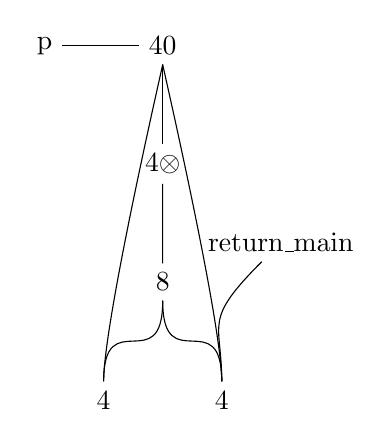
\begin{tikzpicture}[edge from parent path= {(\tikzparentnode.south) .. controls +(0,-1) and +(0,1) ..  (\tikzchildnode.north)}]
		\draw (-1.5,0) node (p) {p}; 
		\draw (1.5,-2.5) node (ret) {return\_main};
		\draw (0,0) node (dag) {40} 
		child {node {4$\otimes$}}
		{ child {node {8}} 
		{ child {node {4}}
		child {node {4}} 
		}
		};
		\draw (dag) .. controls +(0,-0.25) and +(0,1) .. (dag-1-1-1);
		\draw (dag) .. controls +(0,-0.25) and +(0,1) .. (dag-1-1-2);
		\draw (ret) .. controls +(-1,-1) and +(0,1) .. (dag-1-1-2);
		\draw (p) .. controls +(1,0) and +(-1,0) .. (dag);
	\end{tikzpicture}
\end{minipage}
	}
\label{fig:ASI}
\caption{Input and Output of ASI}
\end{figure}

\subsection{Aggregate Structure Identification (ASI)}

ASI is a flow-insensitive algorithm to identify the structure of
aggregates (arrays, structs) in a program.
It interprets the data-access constraints it is given by the VSA and
emits DAGs (Directed Acyclic Graphs) describing the structure of
aggregates used in a program.
	
The easiest way to understand the idea of ASI is to look at an example
input and output.  \callout{Figure \ref{fig:ASI-DAC}} shows the example input that
is generated by VSA for the example given in \callout{Figure \ref{fig:ex-loop}}.
The first two lines describe the assignment of the four byte constants
(\verb+const_1[0:3]+ and \verb+const_2[0:3]+) to the elements of the
structs (\verb+[0:3]+ and \verb+[4:7]+) stored in the array
(\verb+p[0:39]\5+). The third line describes that the bytes four to
seven of the array (\verb+p[4:7]+) are returned by the function
(\verb+return_main[0:3]+).

ASI then generates a DAG describing the layout of the aggregates. For
the example the DAG is shown in \callout{Figure \ref{fig:ASI-DAG}}. A 40 byte variable
called \verb+p+ is subdivided into two variables of 4 bytes length and
an array part consisting of 4 elements of 8 bytes each, which are also
subdivided into two 4 byte variables. One of the 4 byte variables of
\verb+p+ is returned by the \verb+main+ function. 


\begin{figure*}[!t]
	\centering
	\subfloat[Local Variables]{\includegraphics[width=\textwidth]{fig-1}}\\
	\subfloat[Heap Variables]{\includegraphics[width=\textwidth]{fig-2}}
	\caption{Analysis of Example Programs Using \mbox{DIVINE}}
	\label{fig:examples}
\end{figure*}
\subsection{Putting it together}
\enlargethispage{2\baselineskip}

This subsection describes why a single run of VSA and ASI is not sufficient
for a complete analysis of a program's variables and how a loop can be
constructed, which will solve the problem of nested structs.
\begin{figure}[htb]
	\lstset{language=C}
	\begin{lstlisting}
		struct B { int i; };
		struct A { struct B *pb; };
		struct A *pa;
	\end{lstlisting}
	\caption{Example Structures}
	\label{fig:ex-struct}
\end{figure}

For the example given in \callout{Figure \ref{fig:ex-loop}} a single run of the
semi-naïve algorithm, followed by VSA and ASI, was sufficient to recover
all of the programs \mbox{a-loc}s.
\callout{Figure \ref{fig:ex-struct}} shows two structs \verb+A+ and \verb+B+.
Struct \verb+A+ contains a pointer to \verb+B+ as its element. Given
such a constellation, a single run of VSA and ASI would only discover
the element of \verb+A+, but it would not be able to discover
information about the layout of the struct \verb+B+. In this example a
second round of VSA and ASI would discover the layout of \verb+B+.
To solve the problem of \mbox{a-loc} recover for nested structs in general it
is necessary to construct a loop in which VSA and ASI are run until a
fix-point is found.


\begin{figure}[htb]
	\begin{enumerate}
		\item %semi-naïve: env, vsa:cfg,env -> env
			Run the semi-naïve algorithm to find initial \mbox{a-loc}s.
		\item %gen-dac: env -> dac
			Generate data-access constraints for the \mbox{a-loc}s.
		\item %asi: dac -> DAG
			Run ASI to refine the \mbox{a-loc}s.
		\item %vsa:  cfg, env -> env (use indirec-mem-ref)
			Run VSA to find new possible value sets.
		\item %loop 2 until fixpoint
			Loop starting at 2.\ until the set of \mbox{a-loc}s does not change.
	\end{enumerate}
	\caption{\mbox{DIVINE} Loop}
	\label{fig:divine-loop}
\end{figure}


\callout{Figure \ref{fig:divine-loop}} shows the structure of the loop
used by \mbox{DIVINE} to recover the programs \mbox{a-loc}s. 
At first initial \mbox{a-loc}s are generated using the semi-naïve algorithm.
They are then used to find the first aggregates and their \mbox{a-loc}s
possible values using ASI and VSA. The algorithm will then loop on ASI
and VSI until there is no further refinement of the aggregates.
The algorithm will always converge, because ASI can subdivide the
aggregates only up to single bytes in the worst case.


\section{Experiments}
\enlargethispage{4\baselineskip}

The original \mbox{DIVINE} paper \cite{DIVINE} describes the result of the
\mbox{a-loc} recovery on a set of example programs (see \callout{Figure
\ref{fig:examples}}). The \mbox{a-loc}s recovered are compared with the
real program variables and categorized into four categories: matched, if
the \mbox{a-loc} has the same size as the variable; over- or
under-refined, if the \mbox{a-loc} was subdivided into smaller or bigger
parts compared with the actual variable; and incomparable for all other
\mbox{a-loc}s. \callout{Figure \ref{fig:examples}} shows that for all of the
example programs four loops of the algorithm were sufficient to produce
no further changes. The first column shows the results of the semi-naïve
approach, as it is used for the initial \mbox{a-loc}s. All further
columns are the output of the \mbox{DIVINE} algorithm iterations. For
all programs, the loop found additional \mbox{a-loc}s
further refined the under-refined \mbox{a-loc}s or kept
the matched \mbox{a-loc}s. Only for some cases over-refined \mbox{a-loc}s were
generated. For all but one of the programs, heap-variables were
recovered that were not recognized by the semi-naïve approach.

\section{Summary}
\enlargethispage{4\baselineskip}

\mbox{DIVINE} is implemented in a product called Codesurfer/x86. Compared with
the semi-naïve approach \mbox{DIVINE} gives much more refined
\mbox{a-loc}s representing
actual program variables.

The algorithms work for non-x86 assembly languages, development and
release of more analysis applications is still pending.

%\section{Reference}
\begin{thebibliography}{1}
	\bibitem{DIVINE} Gogul Balakrishnan \& Thomas Reps,
		{\mbox{DIVINE}: DIscovering Variables IN Executables},
		VMCAI, 2007
	\bibitem{WYSINWYX-07} Gogul Balakrishnan,
		{WYSINWYX: WHAT YOU SEE IS NOT WHAT YOU EXECUTE},
		Dissertation, University of Wisconsin-Madison, 2007
	\bibitem{WYSINWYX-09} Gogul Balakrishnan \& Thomas Reps,
		{WYSINWYX: What You See Is Not What You eXecute}, TOPLAS, 2009
\end{thebibliography}
\end{document}
